\documentclass{article}
\usepackage{amsmath}
\usepackage{amssymb}
\usepackage{amsthm}
\usepackage[pdftex]{graphicx}
\usepackage{pdfsync}
\usepackage{datetime}
\setlength{\parindent}{0pt}
\pdfpagewidth 8.5in
\pdfpageheight 11in

\newcounter{pbcounter}
\newenvironment{problem}
{\stepcounter{pbcounter}\begin{sloppypar}
	\noindent{\large\bf Problem \arabic{pbcounter}:}
\begin{quote}\itshape}
{\end{quote}\end{sloppypar}}

\newtheorem{prop}{Proposition}[pbcounter]
\newtheorem{lem}[prop]{Lemma}

\title{Programming Assignment 2}
\author{Bertrand Haas}
\date{\today,  \ampmtime}
\begin{document}
\maketitle


\begin{center}
I collaborated with the following people on this assignment:\\
$\bullet$\ Jeff Rabe
\end{center}

\section{Speed Considerations:}
\subsection{Counting for Strassen}
Let's write $ S(n) $ for the number of operations needed to multiply two $ n $ by $ n $ matrices with Strassen's algorithm, and $ R(n) $ for the number of operations using regular matrix multiplications.  
When we multiply two $ n $ by $ n $ matrices by Strassen's algorithm, we first produce matrices $ P_1 $ to $ P_7 $.  
The first four each require one addition (or subtraction) and one multiplication, so they contribute to $ 4 (n/2)^2 + 4\, S(n/2) $.
The last three require each two additions and one multiplication, so they contribute to $ 6 (n/2)^2 + 3\, S(n/2) $.
Then we produce the four resulting block matrices $ K $, $ L $, $ M $ and $ N $ out of $ P_1, \ldots, P_7 $.  
The submatrices $ K $ and $ N $ require three additions each and $ L $ and $ M $ only one each.
So they contribute to $ 8 (n/2)^2 $ operations.
Putting all this together yields:
\begin{equation}
\label{rec_eqt}
S(n) = 7\, S(n/2) + 18(n/2)^2
\end{equation}
For our implementation we can also add the number of operations used to divide $ n $ by two and shift the indices by $ n/2 $.
If we were to consider only the "nice" case of $ n $ being a power of $ 2 $, that's an additional $ +7 $ in the formula above.
\subsection{Regular Counting}
In the regular multiplication we get $ n $ multiplications and $ n-1 $ additions for each entry.  
Therefore the number of operations is $ 2 n^3 - n^2 $.  
Since in our implementation we first set each element to zero and then successively add the multiplicands, we actually count $ n $ additions instead of $ n-1 $, which sinplify the number of operations to $ 2*n^3 $.
\subsection{Solving}
The equation yields:
\begin{eqnarray*}
S(n) &=& 7^k S(\frac{n}{2^k}) + 18(\frac{n}{2})^2(1 + \frac{7}{4} + \ldots + \frac{7}{4^{k-1}}) \\
	 &=& 7^k S(\frac{n}{2^k}) + 6 n^2 (\frac{7}{4}^k - 1) 
\end{eqnarray*}
Assuming $ n $ has the "nice" form $ n = 2^k n_0 $, where $ n_0 $ is the "crossover point", we have $ 7^k = (n/n_0)^{\log 7} $ and $ 4^k = (n/n_0)^2 $.  
Moreover $ S(n/2^k) = S(n_0) $, but since $ n_0 $ is the crossover point, we have to change it to $ R(n_0) $.
So the formula becomes:
\begin{eqnarray*}
S(n) &=& (\frac{n}{n_0})^{\log 7} R(n_0) + 6(\frac{n}{n_0})^{\log 7}n_0^2 - 6 n^2 \\
	 &=& n^{\log 7}\frac{2*n_0^3 + 6 n_0^2}{n_0^{\log 7}} - 6 n^2
\end{eqnarray*}
To optimize the number of operations for large $ n $ we want to minimize the coefficient of the dominant term, $ n^{\log 7} $.
This term simplifies to $ 2(n_0 + 3)/(n_0^{\log(7) - 2}) $;
Diffrentiating with respect to $ n_0 $ and setting to zero we get:
\[
\frac{1}{n_0^{log(7) - 1}} (3 - \log 7)n_0 - 3(\log(7) - 2)
\]
Solving for $ n_0 $ we get $ n_0 = 3 (\log(7) - 2)/(3 - \log 7) = 12.57\ldots $ that we round off to $ n_0 = 13 $.
Plugging it back to the formula above, we find the dominant coefficient equals to $ 4.035\ldots $.
In fact if we look at the graph of the function 
\[
f(x) = \frac{2(x + 3)}{x^{\log(7) - 2}}
\]
(see figure \ref{coef_funct}), we see that it stays below $ 4.3 $ for $ 6 \leq x \leq 33 $, so it allows for quite some variation in choosing $ n_0 $ (at least in that range) without impending too much on the coefficient of the dominant term.
\begin{figure}[h]
\vspace{.2in}
\centerline {
	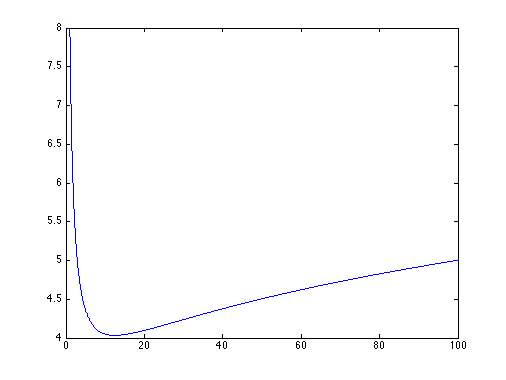
\includegraphics[scale=.6]{coef_funct.png}
}
\caption{The function giving the coefficient of the dominant term. \label{coef_funct}}
%\vspace{.2in}
\end{figure}

\subsection{Experiments}
I reserved some code to compute the best crossover point for $ n $ equal to successive powers of $ 2 $ (from $ 0 $ to $ 1,024 $).  
This is done with the first option set to $ 3 $.  
This part outputs both the crossover point and the number of operations found (2 columns of 11 entries).  
I computed the ratio of the number of operations found to $ n^{\log 7} $ and it seems to converge toward $ 4.03 $ (see figure \ref{rat_coef}), which is exactly the value we found by computation.
\begin{figure}[h]
\vspace{.2in}
\centerline {
	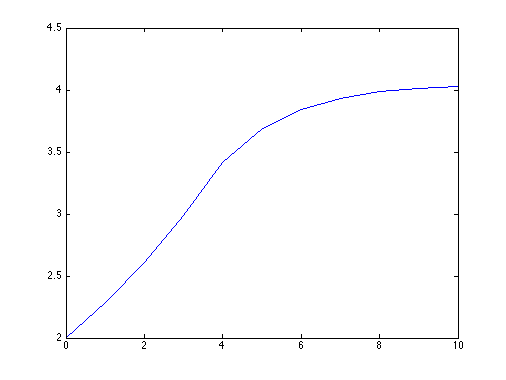
\includegraphics[scale=.6]{rat_coef.png}
}
\caption{The ratio of the number of operations found experimentally over $n^{\log 7} $. \label{rat_coef}}
%\vspace{.2in}
\end{figure}
The graph of the first column, though, seems to indicate the best crossover point is $ 31 $ and not $ 12 $ as we computed (see figure \ref{coef_expm}).
This discrepancy might look a little large and might be understood as comming from several factors: 
\begin{figure}[h]
\vspace{.2in}
\centerline {
	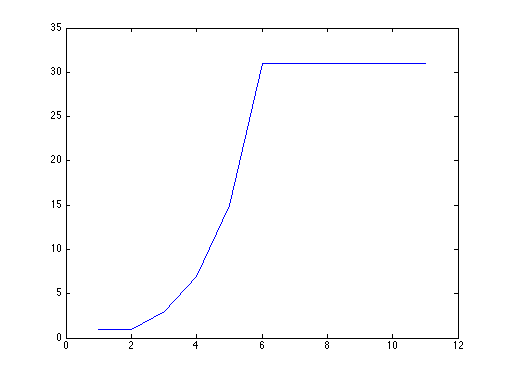
\includegraphics[scale=.6]{coef_expm.png}
}
\caption{The largest optimizing crossover point for each power of $ 2 $ up tp $ 2^{10} $. \label{coef_expm}}
%\vspace{.2in}
\end{figure}
\begin{itemize}
\item The algorithm that outputs $ n_0 $ is greedy, in the sense that it outputs the largest $ n_0 $ found for any given dimension.
And since for simplicity (to avoid adding extra number of operations when a dimension is non-even) I only tested the "nice" case where $ n $ is a power of $ 2 $, we could as well set $ n_0 $ to any value between $ 16 $ and $ 31 $.  
That would yield exactly the same number of operations.  
\item On the other hand, the computation was done with the assumption that it is $ n/n_0 $, and not $ n $ that is a power of $ 2 $, and we found $ n_0 = 13 $ which is not a power of two.  
So the case is slighty different than in the experiment.
\item For similar simplicity concern, in the calculation I disregarded the constant term in \ref{rec_eqt} comming from the $ 7 $ operations on $ n $ and the indices.
This extra term that does not appear for regular multiplications might skew the experimental result toward larger $ n_0 $.
\item Finally the ratio of the number of operations to $ n^{\log 7} $ seems to converge somewhat slowly toward $ 4.035 $.  
We see on figure \ref{rat_coef} that it gets close to it only close to $ n = 2^{10} $ (and crosses $ 4 $ from below only around $ 2^9 $).  
Other non-dominant terms might still weigh in somewhat significantly, and only for $ n $ greater than a larger amount, will the crossover point fall down to close to $ 13 $.
\end{itemize}

\section{Memory Concerns}
In the implementation of Strassen's algorithm for the matrix multiplication $ m_1 * m_2 = m_3 $, the recursive computation of $ P_1, \ldots, P_7 $ might lead to overuse of memory and might stall the program for large $ n $.
It is therefore important to be careful with it.
At the begining of an iteration of Strassen's, we have $ m_1 $ split into the blocks of equal size $ A, B, C, D $, $ m_2 $ split into $ E, F, G, H $ and $ m_3 $ into $ K, L, M, N $.
I start using $ K, L, M, N $ as temporary matrices to compute all the $ P_i $ requiring $ B $.  
Then I can reuse $ B $ and compute with the rest of the free $ K, \ldots, M $ the remaining matrices requiring $ G $.
Now I reuse $ G $, and so on (see the code for the flow).
That way I was able to use only the memory for $ m_1 $, $ m_2 $ and $ m_3 $, that is, $ n^3 $.
Of course, the drawback is that $ m_1 $ and $ m_2 $ are somewhat messed up at the end of the computation.

\section{Other Comments}
To deal with the case where $ n $ is odd, I split the matrix $ m $ into 4 blocks, an $ (n-1) $ by $ (n-1) $ upper-left sub-matrix $ m' $, an $ (n-1) $ by $ 1 $ upper-right sub-matrix (or vector) $ U $, a $ 1 $ by $ (n-1) $ lower-left submatrix (vector) $ V $ and a $ 1 $ by $ 1 $ lower-right submatrix (or scalar) $ W $.
Then I do a Strassen multiplication for the $ m' $, that is, $ m'_1 * m'_2 = m'_3 $, and regular multiplications for the others (only $ O(n^2) $ operations involved).

The testing for the best crossover point was done only with one type of large $ 1024 $ by $ 1024 $ matrix (the number of operations we get really doesn't depend on the values of the matrix--we could as well have everything equal to zero).  
The iterations were done on submatrices increasing in size by a factor of $ 2 $ (see the part of the code for option 3--or "default" in the switch case).
In a previous experiment I computed the best cross-over points and the number of operations for matrices iteratively increasing in size by $ 1 $ up to size $ n = 400 $.  
The pattern for the crossover numbers is very interesting (see figure \ref{coef_400}) and the ratio of the number of operations over $ n^{\log 7} $ also converges toward aproximately $ 4.03\ldots $ (see figure \ref{rat_400}).
However this took a long time to run, and for simplicity and rapidity I switched to increases by a factor of $ 2 $ uo to $ 2^10 $.
\begin{figure}[h]
\vspace{.2in}
\centerline {
	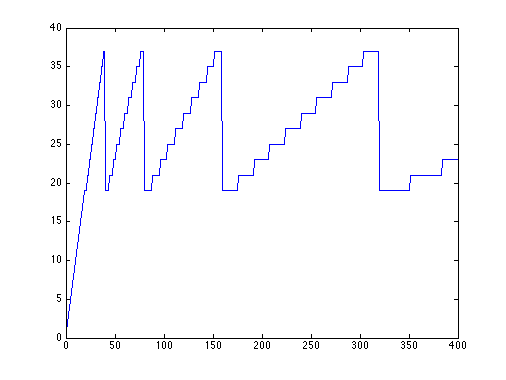
\includegraphics[scale=.6]{coef_400.png}
}
\caption{The largest optimizing crossover point for $ n = 1, \ldots, 400 $. \label{coef_400}}
%\vspace{.2in}
\end{figure}
\begin{figure}[h]
\vspace{.2in}
\centerline {
	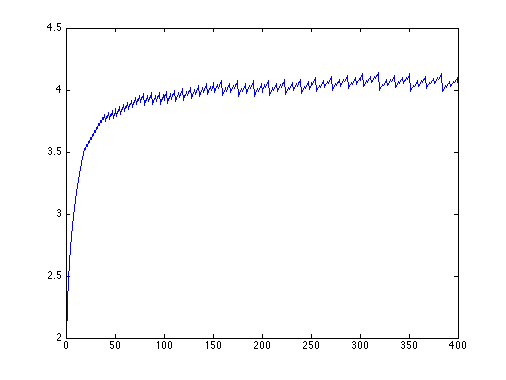
\includegraphics[scale=.6]{rat_400.png}
}
\caption{The ratio of the number of operations over $ n^{\log 7} $ for $ n = 1, \ldots, 400 $. \label{rat_400}}
%\vspace{.2in}
\end{figure}

I included also some C code (in file genmat.c) to generate random matrices.

\end{document}
